% Chapter 4

\chapter{Methodology} % Methodology

\label{Chapter4} % 

From our preliminary analysis we have seen that listening habits, at an aggregate level, follow a strong daily usage pattern. However at an individual user level these patterns are not as strong. In this section we discuss the different methods , of increasing complexity, that were evaluated.

The methods are:

\begin{itemize}
	\item Beta-Binomial model
	\item Epsilon intensive loss function
	\item RBF Regression
	\item Recurrent Neural Networks
\end{itemize}

We start with discussing the data preparation that was performed in order to perform the analysis as well as the evaluation criteria. We then discuss each of the methods.

\section{Data Preparation}

The analysis was carried out in Python (via Jupyter notebooks) running on Ubuntu. The raw data consisted of timestamp of when a song was played and a user ID. These were loaded as-is into a SqlLite3 database. The methods themselves utilized a mixture of scikit learn, Tensorflow, and GPFlow.

UserIDs were then converted to integer (e.g. 'User0005' became '5') and a period table was defined of n minute intervals to which all timestamps could be mapped to. n was chosen to be 30 although it is possible to re-run the analysis for other levels of granularity.

More significantly the data, which contained entries for the times at which each user listened to music, was supplemented with all the times they did \emph{not} listen to music, between their date of their first and last play. As can be imagiend this increased the size of the dataset signifciantly from <> rows to <> rows.

This was necessary in order to evaluate the success of the models in predicting when users would like to listen to music vs. when they would not. From here the data was modelled in two different ways. 

THe second method of modeling the data retains the temporal aspect and is inline with times-series approaches. The data was structure into the following features: PeriodID, UserID, HrsFrom6pm, isSun, isMon, isTue, isWed, isThu, isFri, isSat, t, t1, t2, t3, t4, t5, t10, t12hrs, t24hrs, t1wk, t2wks, t3wks, t4wks.

The first two are self-explanatory. HrsFrom6pm was chosen as based on the preliminary analysis 6pm appeared to be the peak listening time for the population as whole (see next chapter) and was calcuated as the absolute number of hours, in either direction, from 6pm. Days of the week were codified into a one-hot vector notation, and t ... t4wks represent whether or not a user listened to music in the current period, in t minus 1 period, ... t minus 12 hours ago, all the way through to t minus 4 weeks ago.

In this way, for each play or non-play we capture a snapshot of the history up to that point. 4 weeks was chosen as the history length as it was felt to be an adequate amount of time to capture the signals that would help predict a play event.

\section{Test dataset}
 
Two types of test data were selected. The first was a hidden periods test set, formed through random selection of random months from the training dataset and holding them back. 

For simplicity future periods after this month were kept in the training dataset, although it is acknowleged that this does not reflect the real world in which future periods would not be available.

The second method was to hold back the entire history of 10 randomly selected users. This would allow us to assess how well the model performs with new users. Note however that even here data earlier than 1 months history was excluded in order for the time-series based methods to have enough history for the time series base methods to work. Dealing with a lack of information on new users is known as the cold-start problem and in this case the prior probabilities as gathered in the BFreq model would be one way of estimating the liklihood of listening to music. We will touch upon this briefly in the next chapter.

The output field for all but the RNN model was a one dimensional vector consisting of $y = \epsilon (0,1)$.

In the case of the RNN model one-hot encoding was used such that $y \epsilon ([0,1],[1,0])$. This was purely a Tensorflow design choice (as it allows the model to be easily extended to a multi-class use case should the need arise).

\section{Evaluation critera}

The main evaluation criteria across all models was precision, recall, and f1-score. These are common metrics used in information retrieval. 

Precision (P) is defined as the number of true positives  ($T_p$) over the number of true positives plus the number of false positives ($F_p$). A true positive in this case is predicting that user plays or does not play music and being correct.

$$P = \frac{T_p}{T_p+F_p}$$

Recall (R) is defined as the number of true positives ($T_p$) over the number of true positives plus the number of false negatives ($F_n$). For example if we predicted 100 plays correctly but there were in fact 110 plays in the dataset, then recall would be 100/110 = 91%.

$$R = \frac{T_p}{T_p + F_n}$$

A high precision score does not necessarily mean a high recall score, and often an improved precision can mean a lower recall (making fewer guesses but with a higher degree of accuracy). We place this in the real world context and ask what we value. For a home audio device, suggesting music when the user does not want to listen to music would carry a higher cost than not suggesting music when a user does not wants to listen to music. Therefore precision is more important than recall. Of course a high score in both is ideal, and this is captured by the F1 score.

F1 is defined as the harmonic mean of precision and recall.

$$F1 = 2\frac{P \times R}{P+R}$$

\chapter{Methodology} % Methodology

Several models were evaluated. As the goal of the research was to evaluate the effecitvneess of different methods, extensive feature engineering beyond what has been described was not performed. 

Random salection of test periods was perormed each time any of the results were run, while test users were selected at the outset and kept fixed throughout.
 
\section{Beta-Binomial model (BetaBin)}

The Beta-Binomial model is one of the most simple Bayesian inference models, and has a tractable solution.

We define our liklihood, the probability of a user listening to music, as a binomial distribution, where $k$ is the number of plays in a given period, $n$ is the sum of plays and non-plays, and $\theta$ is the unknown probability parameter for the binomial distribution.. 

$${n \choose k}\,p^{k}(1-p)^{n-k}$$

Here our period, or rather timeslot, is the set of half hourly intervals within an entire week (so 24*2*7=336 timeslots). This is different to the time-series approach we adopt for the latter methods. Here the frequency of plays and non-plays are dervied at the userID, timeslot level, where timeslot is a string concatenation of weekday, hour of day, and start minute of period. 

Our prior is Beta distribution of $\theta$:

$$p(\theta)=\frac{x^{\alpha-1}(1-x)^{\beta-1}} {B(\alpha,\beta)}$$ where
$$\mathrm {B} (\alpha ,\beta )={\frac {\Gamma (\alpha )\Gamma (\beta )}{\Gamma (\alpha +\beta )}}$$

A the Beta distribution is a conjugate prior to the Binomial the formula can be reduced to: $Beta(\alpha+P, \beta+Q)$ where P is the count of plays and Q is the count of non-plays.

Our prior parameters, $\alpha$ and $\beta$, are dervied from the training set, with an estimate for each half-hourly time period. 

Finally we convert the probabilites into a binary outcome by optimizing for a threshold $\lambda$ at which we predict a play event.

The remaining models adopted a time-series approach. Let $E = 1$ represent a Play event, and $E = 0$ a non-play event. $t$ is the half-hourly time period we are predicting for, and $h$ represent the half-hourly history. We therefore seek to calculate the probability of an event in the currenty time period, given the history of events, $p(E_t \mid E_h)$, for each individual user. 

\subsection{Binary Logistic Regression (LogReg)}

Here our model is:
$p(E_t = 1 | E_h) =  \sigma(w'x + b)$

where $w'$ is a weight matrix transpose, and x is our input features, and b is a constant. 

\subsection{Linear SVM Regression}

A linear SVM regression model is characterized by the Epsilon Intesive loss function \parencite{Vapnik}. By modifying the loss function to ignore errors that are within a certain margin, $\epsilon$m helps prevent overfitting.

Our objective becomes to minimize:

$$max(0,\left\| (y_i - w_i x_i - b) - \epsilon \right\|)$$


\subsection{Non-Linear RBF Regression}

Here we extend a regression model to include a Gaussian RBF kernel:

$$p(E=1)=b+\sum^N_{i=1}w_iRBF(x,x_i)$$

where RBF is:

$$K(\mathbf {x} ,\mathbf {x'} )=\exp \left(-{\frac {\|\mathbf {x} -\mathbf {x'} \|^{2}}{2\sigma ^{2}}}\right)$$

Note that the actual implementation in Tesnorflow made use of the fast computation of the RBF kernel as defined by McClure \parencite{TFCookbook}. The restated method has a hyperparameter $\gamma$ that takes the place of $2\sigma^2$ which requires calibrating.

The Kernel allows us to solve for non-linear problems by transforming our x values to a high dimensional space. Note that performing such calculations is computationally intensive and as such mini-batch training will be performed with a batch size of 2000 and 5 iterations of the dataset. (Rows of more than 5000 tended to cause memory errors, and iterations beyond 5 showed minimal or no decrease in loss)

\subsection{Gaussian Processes}





\hfill \break
\hfill \break
\hfill \break
\hfill \break





\subsection{Recurrent Neural Networks}

Recurrent nets are a type of artificial neural network designed to recognize patterns in sequences of data, such as text, genomes, handwriting, the spoken word, or numerical times series data emanating from sensors, stock markets and government agencies. Whereas a Feed-Forward network has input nodes, hidden layers, and an output layer, with data flowing in one direction only; RNNs allow for the hidden state from timestep of the neural net to be an input into the next.

\begin{figure}[h!]
	\centering
	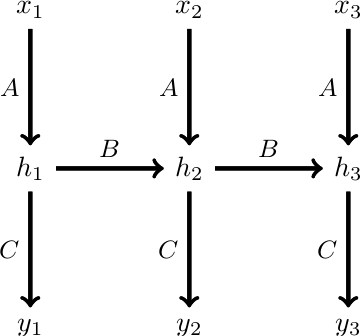
\includegraphics[width=3cm, keepaspectratio,]{fig007.jpg}
	\caption{RNN with 3 timesteps}
	\label{fig:fig7}
\end{figure} 

An LSTM is an extension of an RNN model in which the hidden layer which is transmitted across time steps is further divided into four layers that interact in a way as to learn what information to retain, and what information can be thrown away \parencite{Olah}. 

\begin{figure}[h!]
	\centering
	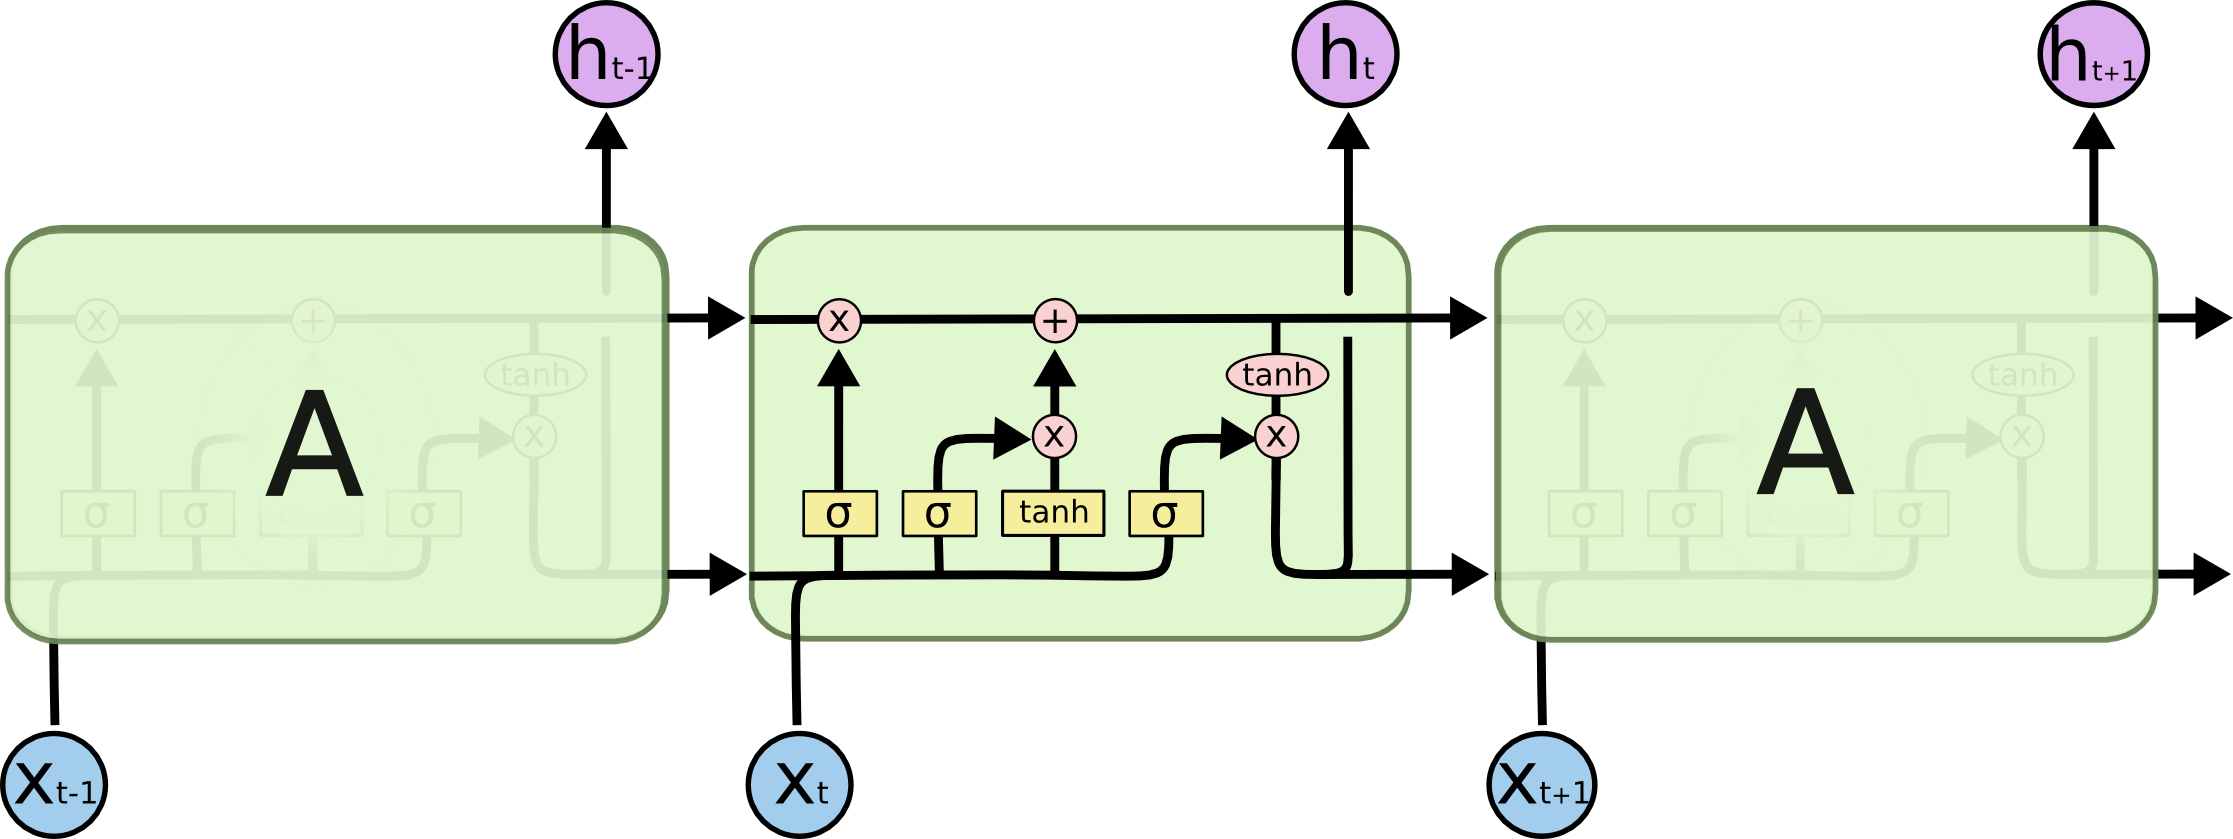
\includegraphics[width=5cm, keepaspectratio,]{fig008.png}
	\caption{LSTM}
	\label{fig:fig8}
\end{figure} 
